\documentclass[a4paper, 11pt]{article}

\usepackage{natbib}
\bibliographystyle{agsm}
\setcitestyle{authoryear,open={(},close={)}}

\usepackage{fontspec}
\setmainfont[Ligatures=TeX]{Lato Light}

\usepackage{graphicx}
\usepackage{wrapfig}

\linespread{1.05}

\makeatletter
\renewcommand{\maketitle}{
\begin{flushright}
{\LARGE\@title}

\vspace{50pt}

{\large\@author}
\\\@date 
\vspace{40pt}
\end{flushright}
}
\renewcommand{\@seccntformat}[1]{}
\makeatother



\title{\textbf{Funding in the Platform Economy}\\Agency Theory and Venture Capital Finance}


\author{\textsc{Ans Vaessen}
\\13009722
\\{\textit{Entrepreneurship and Innovation}}}

\date{\today\\
word count: 3037}

%%%%%%%%%%%%%%%%% START %%%%%%%%%%%%%%%%%%

\begin{document}
\maketitle

\begin{abstract}
moet ik nog doen.
\end{abstract}



\vspace{30pt} % Some vertical space between the abstract and first section

\section*{Introduction}


Within the sharing economy new businesses like Uber, AirBnB, GetYourGuide and Brewdog new business models emerge. From a closed business model to a more open model that uses online platforms to connect customers with service providers or products. These four businesses not only use new busies models, they also qualify as unicorns, ventures that are worth one billion dollars or more \citep{TiddBessant}. Do these new business models impact the way start-ups are funded and what is the influence of this peer-to-peer sharing economy concept on the agency theory?

\section{Small and Medium Enterprise Businesses Start-up Finance}

These new businesses or ventures are different from the more traditional business because they develop a product that is not ready for the market, because it is still in a developing phase or the market is not aware of this new product. Therefore, \cite{TiddBessant} argue funding of a new business differs because it can not follow a normal cash flow from early sales. Also the initial funding needed, depends on the sort of business, for example a biotechnology start-up needs more funding than a software start-up \citep{TiddBessant}. The sort of funding not only depends on the sort of business. It also depends on how far the business is developed. There are different models to explain the cycle a new business is going through. All the models follow more or less the same line. Figure \ref{fig:graph1} below shows shows how a venture evolves from a seed (an initial idea) to the next stage and when the idea turns out to be successful it moves on to the following stages unil it finally exits as an IPO, acquisition or merger.

\begin{figure}[h!]
    \centering
    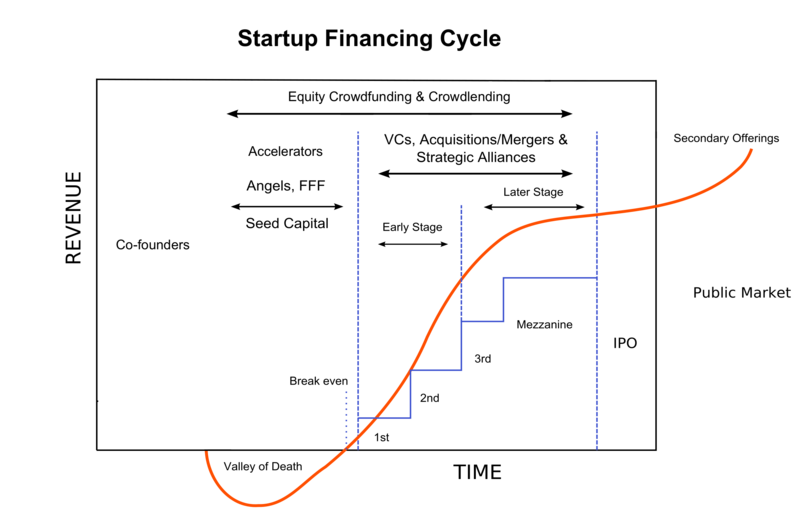
\includegraphics[width=0.9\textwidth]{FinCycle.png}
    \caption{Start-up finance cycle \cite{wiki}.}
    \label{fig:graph1}
\end{figure}

Every stage also brings its own problems or challenges. The first stage the valley of death is hard to get through and most business fail in this so called seed stage. If a business gets funds at this stage it is ofthen through family and friends, crowdfunding, accelerators, seedcamp and sometimes angels, but not venture capitalists \citep{TiddBessant}. If the venture survives, it needs more funding and this funding often comes from outside the company. \cite{casson2008oxford} states that the main source of funding for small firms are the more traditional institutes like banks, however young high tech businesses lack the track record or collateral required for such debt funding. So in order to grow the venture they will look for outside equity funding.

This essay will focus on this form of finance in relation to the agency theory and how new business models, like open business models, platform technology or sharing economy influence this funding.

\section{Equity Funding}

Small and medium entrepreneurs will often need outside funding after the first initial phase, which is often funded with their own savings and/or money from family and friends. Once a business wants to grow further past this initial start, it needs more funding and traditional investors like banks are not likely to invest because of the uncertainty and high, inherent, risk in new businesses \citep{Osnabrugge2000}. So instead of going to the bank an entrepreneur can choose to find a venture capitalist.

\subsection{Venture Capital}

In the Oxford Handbook of Entrepreneurs the following definition is used:

\begin{quote}
"Venture capital investment consists in the purchase of shares of young, privately held companies by outsiders for the primary purpose of capital gain" \citep[P.355]{casson2008oxford}.
\end{quote}

The capital injections are mostly done in stages \cite{TiddBessant} for example distinguishes four stages because every stage of development needs different conditions and financial needs. As mentioned when discussing Figure \ref{fig:graph1} in the initial stage, money will come mostly from savings, family and friends, however later on they need larger amounts of money. The idea is, a venture capitalist invest in a high risk business after the initial stage, yet still early enough to sell the shares later for high profits when the company exits \citep{TiddBessant}.

Venture Capital has a couple of advantages for the entrepreneur. It does not require tangible assets that banks ask for as a security. The investments are paid back when the company succeeds and is therefor more flexible and as stated by \cite{casson2008oxford} an other important advantage is the expertise the venture capitalist can bring into the company. However there is a downside as well. The venture capitalist wants part of the value of the company in return and also want control in how the company is run \citep{casson2008oxford}.

Other ways to get more security for the venture capitalist is when a start-up has a patent for the new product or service.
\cite{nadeau2011innovation} shows there is evidence that protection of intellectual property rights will improve the changes of a successful exit for the business and therefor it will be easier to attract venture capital.

 \cite{Roma} points that another way to attract the interest of professional investors is, when entrepreneurs enjoy a large network that can stimulates trust. This can be accomplished through crowdfunding for example.


The venture capitalist wants control to make sure the outcome is what is aimed for, a profit when the company exits. The venture hardly ever provides a positive cash flow before a liquidity event (exit), the most common forms of exits are going public in a Initial Public Offerings (IPO) or a private sale of the venture to an other firm, Merger and Acquisition (M\&A) \citep{nadeau2011innovation}.

Venture capitalists can invest their own money, but also raise funds from other investors (banks, pension funds or insurance companies) the so called fund providers \citep{casson2008oxford}.

Venture capital is well known but there are other ways of equity funding namely business angels, crowdfunding, incubators and accelerators.

\subsection{Business Angels}
These are individuals that fund unlisted companies without having any family or friend connection, they not only invest capital. \cite{politis} adds that besides their money they also bring theirbusiness skills, personnel networks and expertise. In figure \ref{fig:graph1} this is shown as a funding in the seed stage, but they can also play an important part in later stages of the company.


\subsection{Crowd Funding}
Crowd funding is regarded as a relatively new way of gaining outside capital. Mediated by a web portal a project or company can attract multiple nonprofessional investors \citep{TiddBessant}. \cite{belleflamme} distinguishes two forms of crowd funding either by pre order or advanced payment in exchange for a share in future profit. The author adds that crowdfunding  remains relatively small compared to other sources. Especially the pre-selling reshaped the funding life-cycle we saw earlier, \cite{bella} even states this could disrupt venture finance, because the company can sell millions of products without needing initial funds to produce them.

\subsection{Incubators and Accelerators}
Programmes to help with your business an accelerators can help growth of an existing company focus on scale. Whereas an incubators helps people with an idea to build a company and focuses on innovation. An accelerator programme will make a small seed investment in return for equity. The entrepreneur receives funding but more importantly access to mentor-ship network to grow their business faster \citep{forrest}.

Whatever source of funding is used their is always an asymmetry in information between the lender and company, this is reffered to as the agency theory.

\section{Agency Theory}

In most companies that make use of outside funding there is a separation between
the owner of the business (agent) and the lender or investor, this can be a
bank, venture capitalist or angel investor (principal). The principal wants
security in return of the investment to ensure the money invested is used well
and the principal is not harmed by actions of the agent \citep{jensen1976theory}.

The risk is in the asymmetry of information between the agent and the principal. Often the
agent has information about the firm and its day to day operations that is not
available to the principle. This can harm the principal if the agent uses the
information to benefit him or herself over the benefits of the principal
\citep{Osnabrugge2000}.

Furthermore, there is also an asymmetry in information between the fund provider and the venture capitalist \citep{casson2008oxford}. ... nog een zinnetje....

Looking at crowdfunding principal-agent theory can be applied \cite{chaney} calls this inverted agency relationship, were consumers have some ideas about products to put on the market as principals and companies giving shape to these ideas as agents. So as with funding from venture capitalist, the company has to share its information and creative decision making with the consumer, \citep{chaney} unfortunately does not mention what this relationship implies for the next phase when a company looks for larger investment from, for example, venture capitalist.



\subsection{Contracts}
\cite{Osnabrugge2000} continues to describes it is difficult for the principal to verify the information and that the two parties can have different views on how to run the company best, so they set up contracts to limit these so called agency costs.


These contracts are to tackle this problem. \cite{jensen1976theory} defines an agency relationship as contract in which both parties agree that the principal delegates some authority on decision making to the agent to reduce the agency cost of informing each other on every detail, at the same time both parties agree on criteria to asses the performance of the agent.

Further research shows there is a difference in contracts. To form an optimal contract can be very costly so their is also the incomplete contract. The first optimal contract is formulated to predict the foreseeable future and follows behavior vs outcome, screening and analysis are important to reduce the asymmetries of information between the principal and agent \citep{Osnabrugge2000}. The latter incomplete contract, presumes contract are always incomplete and it is better to invest in involvement and relationship with the agent  \citep{Osnabrugge2000}. The author shows in his research that business angels prefer the incomplete contracts and venture capitalist choose to invest more in the screening in the pre-investment phase in order to gain more security.



\subsection{Staging and Syndication}
As mentioned earlier funding is done in stages and to grow a business further it is possible that in a next round other venture capitalists in invest in the same company, this is called syndication of investment \citep{casson2008oxford}. Staging reduces agency cost as the venture capitalist can leave the venture if it is not performing well enough and furthermore it is a way to get to know each other better before taking the next step \citep{colombo2016open}. There are different reasons for syndication  \cite{colombo2016open} points out three reasons for syndication. Firstly to reduce risks, secondly to improve selection of high-quality ventures, the quality is checked by each syndicate member and thirdly to bring in different skills, expertise and networks in order to help the venture and add more value than with just one business angel or venture capitalist \citep{colombo2016open}. 


\section{New Business Models}
In the past decades their is a trend towards more open innovation and open businesses. Another trend is the sharing economy and platform models, some of the new businesses make extensive use of these models and change the game for funding and information asymmetry.

\subsection{Open Business Models}

Open business models are businesses that use external sources of technology and knowledge or sharing their own knowledge including intellectual properties with others outside \citep{chesbrough2007companies}.
As \cite{colombo2016open} argues that the growing popularity of open innovation is not researched enough most models apply on closed business models. As \cite{colombo2016open} points out there are many forms of open business models, one of them is Open Source Software. Another is the sharing economy making use of platform business models.


\subsection{Sharing Economy and Platform Business Models}
A lot of companies build their open business model by using the online community. These business depend on the engagement of their community for value generation and expanding their business \citep{colombo2016open}. To share information the new ventures make use of platforms bringing together the producer and consumer. From simple retailing the market moved to online exchange of accommodation, information, transportation via platforms like Airbnb, GetYourGuide and Uber to name a few. There are many definitions but according to \cite{investopia} this economic model is frequently defined as peer-to-peer (P2P) based activity of acquiring, providing or sharing access to goods and services that are facilitated by a community based on-line platform.



\section{Role of Venture Capital for Platform Business Models}

\cite{colombo2016open} explains that venture capitalist are best suited to deal with open business models, they are high risk and venture capitalist can cope well with information asymmetry. In closed business models for software, entrepreneurs often rely on patents to protect their product and prevent others to copy it and to capture the value by licensing the product. For example software code, when entrepreneurs adopt an open business model the value comes from selling better versions or extra services on top of the free software \citep{colombo2016open}. In his reseach \cite{colombo2016open} looked at rounds of investment to determine in how many stages a business was funded and for syndication he looked at the number of venture capitalists investing each round. In his paper the focus is on open source software companies, not platform models.


There are several stories about these new business models and their way to the public market. To get a better idea and to see if there are any pattern comparable with \cite{colombo2016open} research towards staging and syndication, four cases of platform business models will be discussed briefly.


\subsection{Uber}

The company is a platform which connects drivers with people who are looking for a ride. \cite{griswold} writes how UberCab was founded when a few friends came up with the idea in 2009 and launched the app in 2010,they were forced to change their namer to UBER rolled out their company to other cities and countries.

The competition grew and UBER spent a lot of money buying out the competition, especially in China and India. Uber’s regional rivals in Asia had powerful investors as well like Softbank and Alibaba. Uber won the American market but not the Asian one and sold their China operations. Uber is continuously unprofitable. In 2017 Uber lost over \$4 billion and only was profitable in 2018 because it sold their international operations. They admit they still rely on discounts for consumers and driver incentives and is planning to continue these subsidies for customers when they went public in April 2019. With going public they hope to convince prospective investors that they can be the next big company \cite{griswold}.

\subsection{AirBnB}
The company, AirBnB developed a platform website connecting people who look for accommodation with people who want to rent-out a accommodation. A good example of an open business model were the input comes directly from the providers and sharing this information on a platform. The company was founded in 2008 and made use of an incubator programm, Y-Combinator, they invested \$20.000 seed money before raising money from various angel investors, and venture capitalists \citep{mazzarini}. In 2018 the company was vallued at \$31 billion \citep{mazzarini}.

\subsection{GetYourGuide}
GetYourGuide is a booking platform for tours, attractions and activities founded by a group of students who came up with the idea after a trip to China \citep{getyourguide}. The first years the company survived on bootstrapping its first seed round in 2012 raised \$2 million. This was followed by a Series A in early 2013 when it raised \$14 million \citep{webintravel}. Now they are in a late stage venture and vallued at \$1.78 billion \citep{techcrunh}. 

\subsection{Brewdog}
This is a brewery and the company might not look like a platform but are called a new-age business model, starting as a crowdfunded business in 2007 by selling shares as Equity Punk, even with new investment rounds they kept the crowdfunding model, Equity Punk partners could vote in advance on the proposed TSG investment \citep{danziger}. Accoridng to the owner of Brewdog their ultimate end game is to go public and get those that invested in shares get real monetary value, the valluation in 2017 was \$1.24 billion \citep{danziger}.

\section{Is There a Pattern?}

Out of these four cases a couple of observations can be made as we can see in Table 1 using the data from \citep{crunch} to make a comparison between the 4 companies.

\begin{table}[h!]
    \begin{tabular}{|p{2cm}|p{2.2cm}|p{2cm}|p{2.2cm}|p{2.2cm}|}
\hline
                & Uber & AirBnb & BrewDog & GetYourGuide        \\
\hline
Seed            & Savings & Incubator & Crowdfunding & Bootstrapping \ and 2 million \\
\hline
Funding Status  & IPO\newline{}after series G & Late Stage Venture\newline Series F & Equity\newline Crowdfunding & Late Stage\newline Venture Series E \\
\hline
Funding Rounds  & 23 & 16 & 12 & 8 \\
\hline
Number of Investors & 99 & 53 & 6 & 23 \\
\hline
\end{tabular}
\label{tab:compare}
\caption{Compare.}
\end{table}


It is only a brief look at four companies and in no way represents any out come but comparing with and more research necessary
tabel


\section{agency theory and information asymmetry in platforms}
As explained earlier the agency theory in regards to the investor and the company explains how there is a asymmetry in information. There is plenty of information about the asymmetry of information between seller and buyer on the online market and how peer-to-peer business closes this gaps with reviews about both the customers and the producer or service provider. How ever I have not found any research about the impact of this more open new business model on the information asymmetry towards the investors. Only  \cite{colombo2016open} briefly touches on subject by assuming that when more are involved one can assume the information is even more asymmetrical.




Different companies different stages hard to compare but interesting to see the funding is




\section{Conclusion}

And to conclude one could say bla bla bla


%% disable some things
\renewcommand{\textbf}{}
\renewcommand{\bf}{}
\bibliography{biblio}{}
\end{document}
